\documentclass{article}
\def\pgfsysdriver{pgfsys-tex4ht.def}
\usepackage{pgf}
\usepackage{amsmath}

\usepackage{tikz}
\usetikzlibrary{scopes,positioning}
\begin{document}

\def\iangle{35} % Angle of the inclined plane

\def\down{-90}
\def\arcr{0.5cm} % Radius of the arc used to indicate angles

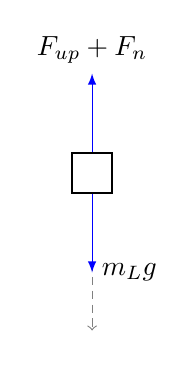
\begin{tikzpicture}[
    force/.style={>=latex,draw=blue,fill=blue},
    axis/.style={densely dashed,gray,font=\small},
    M/.style={rectangle,draw,fill=lightgray,minimum size=0.5cm,thin},
    m/.style={rectangle,draw=black,fill=none,minimum size=0.5cm, thick},
    plane/.style={draw=black,fill=blue!10},
    string/.style={draw=red, thick},
    pulley/.style={thick},
]

\tikzstyle{matrix of math nodes}=[%
  matrix of nodes,
  nodes={%
   execute at begin node=$,%
   execute at end node=$%
  }%
]


    %%%

    % Free body diagram of m
    \node[m] (m) {};
    \draw[axis,->] (m) -- ++(0,-2) node[left] {};
    {[force,->]
        \draw (m.north) -- ++(0,1) node[above] {$F_{up} + F_{n}$};
        \draw (m.south) -- ++(0,-1) node[right] {$m_Lg$};
    }



\end{tikzpicture}

\end{document}
